\documentclass{article}
\usepackage[utf8]{inputenc}

%
% Homework Details
%   - Title
%   - Due date
%   - Class
%   - Section/Time
%   - Instructor
%   - Author
%
\newcommand{\hmwkTitle}{Homework Template}
\newcommand{\hmwkDueDate}{\today}
\newcommand{\hmwkDueTime}{11:59 am}
\newcommand{\hmwkClass}{CLASS 100}
%\newcommand{\hmwkClassTime}{Section A}
%\newcommand{\hmwkClassInstructor}{Professor Isaac Newton}
\newcommand{\hmwkAuthorName}{\textbf{Katie Mummah} \and \textbf{Other Name}} %\and \textbf{Davis Josh}}

%
% Use Packages
%
\usepackage[acronym,toc]{glossaries} %%%% Acronym/glossary support
\usepackage [english]{babel}
\usepackage [autostyle, english = american]{csquotes}
\MakeOuterQuote{"}
\usepackage[flushleft]{threeparttable}
\usepackage[margin=1.0in]{geometry}
\usepackage[plain]{algorithm}
\usepackage{algpseudocode}
\usepackage{amsfonts}
\usepackage{amsmath}
\usepackage{amssymb}
\usepackage{amsthm}
\usepackage{amsxtra}
\usepackage{array,epsfig}
\usepackage{biblatex}
\usepackage{booktabs} % nice rules (thick lines) for
\usepackage{caption}
\usepackage{color}
\usepackage{empheq}
\usepackage{enumerate}
\usepackage{enumitem}
\usepackage{extramarks}
\usepackage{fancyhdr}
\usepackage{float} % This can force an image or a chart in place
\usepackage{gensymb}
\usepackage{graphicx} % allows inclusion of graphics
\usepackage{hyperref}
\usepackage{import}
\usepackage{listings}
\usepackage{longtable} %allows for tables to go onto a second page
\usepackage{mathrsfs}
\usepackage{microtype} % improves typography for PDF
\usepackage{nicefrac}
\usepackage{nuc}
\usepackage{physics}
\usepackage{subcaption}
\usepackage{tikz}

\addbibresource{bibliography.bib}
\hypersetup{
    colorlinks,
    citecolor=black,
    filecolor=black,
    linkcolor=black,
    urlcolor=black
}

%\newacronym{<++>}{<++>}{<++>}
\newacronym[longplural={metric tons of heavy metal}]{MTHM}{MTHM}{metric ton of heavy metal}
\newacronym{ABM}{ABM}{agent-based modeling}
\newacronym{ACDIS}{ACDIS}{Program in Arms Control \& Domestic and International Security}
\newacronym{AHTR}{AHTR}{Advanced High Temperature Reactor}
\newacronym{ANDRA}{ANDRA}{Agence Nationale pour la gestion des D\'echets RAdioactifs, the French National Agency for Radioactive Waste Management}
\newacronym{ANL}{ANL}{Argonne National Laboratory}
\newacronym{API}{API}{application programming interface}
\newacronym{ARE}{ARE}{Aircraft Reactor Experiment}
\newacronym{ARFC}{ARFC}{Advanced Reactors and Fuel Cycles}
\newacronym{ASME}{ASME}{American Society of Mechanical Engineers}
\newacronym{ATWS}{ATWS}{Anticipated Transient Without Scram}
\newacronym{BDBE}{BDBE}{Beyond Design Basis Event}
\newacronym{BIDS}{BIDS}{Berkeley Institute for Data Science}
\newacronym{BOL}{BOL}{Beginning of Life}
\newacronym{BRC}{BRC}{Blue Ribbon Commission on America's Nuclear Future}
\newacronym{CAFCA}{CAFCA}{ Code for Advanced Fuel Cycles Assessment }
\newacronym{CDTN}{CDTN}{Centro de Desenvolvimento da Tecnologia Nuclear}
\newacronym{CEA}{CEA}{Commissariat \`a l'\'Energie Atomique et aux \'Energies Alternatives}
\newacronym{CI}{CI}{continuous integration}
\newacronym{CNEN}{CNEN}{Comiss\~{a}o Nacional de Energia Nuclear}
\newacronym{CNERG}{CNERG}{Computational Nuclear Engineering Research Group}
\newacronym{COSI}{COSI}{Commelini-Sicard}
\newacronym{COTS}{COTS}{commercial, off-the-shelf}
\newacronym{CSNF}{CSNF}{commercial spent nuclear fuel}
\newacronym{CTAH}{CTAHs}{Coiled Tube Air Heaters}
\newacronym{CUBIT}{CUBIT}{CUBIT Geometry and Mesh Generation Toolkit}
\newacronym{CURIE}{CURIE}{Centralized Used Fuel Resource for Information Exchange}
\newacronym{DAG}{DAG}{directed acyclic graph}
\newacronym{DANESS}{DANESS}{Dynamic Analysis of Nuclear Energy System Strategies}
\newacronym{DBE}{DBE}{Design Basis Event}
\newacronym{DESAE}{DESAE}{Dynamic Analysis of Nuclear Energy Systems Strategies}
\newacronym{DHS}{DHS}{Department of Homeland Security}
\newacronym{DOE}{DOE}{Department of Energy}
\newacronym{DRACS}{DRACS}{Direct Reactor Auxiliary Cooling System}
\newacronym{DRE}{DRE}{dynamic resource exchange}
\newacronym{DSNF}{DSNF}{DOE spent nuclear fuel}
\newacronym{DYMOND}{DYMOND}{Dynamic Model of Nuclear Development }
\newacronym{EBS}{EBS}{Engineered Barrier System}
\newacronym{EDZ}{EDZ}{Excavation Disturbed Zone}
\newacronym{EIA}{EIA}{U.S. Energy Information Administration}
\newacronym{EOC}{EOC}{End of Cycle}
\newacronym{EOL}{EOL}{End of Life}
\newacronym{EPA}{EPA}{Environmental Protection Agency}
\newacronym{EP}{EP}{Engineering Physics}
\newacronym{FCO}{FCO}{Fuel Cycle Options}
\newacronym{FCT}{FCT}{Fuel Cycle Technology}
\newacronym{FEHM}{FEHM}{Finite Element Heat and Mass Transfer}
\newacronym{FEPs}{FEPs}{Features, Events, and Processes}
\newacronym{FHR}{FHR}{Fluoride-Salt-Cooled High-Temperature Reactor}
\newacronym{FLiBe}{FLiBe}{Fluoride-Lithium-Beryllium}
\newacronym{GDSE}{GDSE}{Generic Disposal System Environment}
\newacronym{GDSM}{GDSM}{Generic Disposal System Model}
\newacronym{GENIUSv1}{GENIUSv1}{Global Evaluation of Nuclear Infrastructure Utilization Scenarios, Version 1}
\newacronym{GENIUSv2}{GENIUSv2}{Global Evaluation of Nuclear Infrastructure Utilization Scenarios, Version 2}
\newacronym{GENIUS}{GENIUS}{Global Evaluation of Nuclear Infrastructure Utilization Scenarios}
\newacronym{GPAM}{GPAM}{Generic Performance Assessment Model}
\newacronym{GRSAC}{GRSAC}{Graphite Reactor Severe Accident Code}
\newacronym{GUI}{GUI}{graphical user interface}
\newacronym{HE}{HE}{high explosives}
\newacronym{HLW}{HLW}{high level waste}
\newacronym{HPC}{HPC}{high-performance computing}
\newacronym{HTC}{HTC}{high-throughput computing}
\newacronym{HTGR}{HTGR}{High Temperature Gas-Cooled Reactor}
\newacronym{IAEA}{IAEA}{International Atomic Energy Agency}
\newacronym{ICBM}{ICBM}{Intercontinental Ballistic Missle}
\newacronym{IEMA}{IEMA}{Illinois Emergency Mangament Agency}
\newacronym{INL}{INL}{Idaho National Laboratory}
\newacronym{IPRR1}{IRP-R1}{Instituto de Pesquisas Radioativas Reator 1}
\newacronym{IRP}{IRP}{Integrated Research Project}
\newacronym{ISFSI}{ISFSI}{Independent Spent Fuel Storage Installation}
\newacronym{ISRG}{ISRG}{Independent Student Research Group}
\newacronym{JFNK}{JFNK}{Jacobian-Free Newton Krylov}
\newacronym{LANL}{LANL}{Los Alamos National Laboratory}
\newacronym{LBNL}{LBNL}{Lawrence Berkeley National Laboratory}
\newacronym{LCOE}{LCOE}{levelized cost of electricity}
\newacronym{LDRD}{LDRD}{laboratory directed research and development}
\newacronym{LFR}{LFR}{Lead-Cooled Fast Reactor}
\newacronym{LLNL}{LLNL}{Lawrence Livermore National Laboratory}
\newacronym{LMFBR}{LMFBR}{Liquid Metal Fast Breeder Reactor}
\newacronym{LOFC}{LOFC}{Loss of Forced Cooling}
\newacronym{LOHS}{LOHS}{Loss of Heat Sink}
\newacronym{LOLA}{LOLA}{Loss of Large Area}
\newacronym{LP}{LP}{linear program}
\newacronym{MA}{MA}{minor actinide}
\newacronym{MCNP}{MCNP}{Monte Carlo N-Particle code}
\newacronym{MILP}{MILP}{mixed-integer linear program}
\newacronym{MIT}{MIT}{the Massachusetts Institute of Technology}
\newacronym{MOAB}{MOAB}{Mesh-Oriented datABase}
\newacronym{MOOSE}{MOOSE}{Multiphysics Object-Oriented Simulation Environment}
\newacronym{MOX}{MOX}{mixed oxide}
\newacronym{MPC}{MPC}{multi-purpose canister}
\newacronym{MSBR}{MSBR}{Molten Salt Breeder Reactor}
\newacronym{MSRE}{MSRE}{Molten Salt Reactor Experiment}
\newacronym{MSR}{MSR}{Molten Salt Reactor}
\newacronym{NAGRA}{NAGRA}{National Cooperative for the Disposal of Radioactive Waste}
\newacronym{NEAMS}{NEAMS}{Nuclear Engineering Advanced Modeling and Simulation}
\newacronym{NEUP}{NEUP}{Nuclear Energy University Programs}
\newacronym{NFCSim}{NFCSim}{Nuclear Fuel Cycle Simulator}
\newacronym{NGNP}{NGNP}{Next Generation Nuclear Plant}
\newacronym{NWPA}{NWPA}{Nuclear Waste Policy Act}
\newacronym{NMWPC}{NMWPC}{Nuclear MW Per Capita}
\newacronym{NNSA}{NNSA}{National Nuclear Security Administration}
\newacronym{NPRE}{NPRE}{Department of Nuclear, Plasma, and Radiological Engineering}
\newacronym{NQA1}{NQA-1}{Nuclear Quality Assurance - 1}
\newacronym{NRC}{NRC}{Nuclear Regulatory Commission}
\newacronym{NSF}{NSF}{National Science Foundation}
\newacronym{NSSC}{NSSC}{Nuclear Science and Security Consortium}
\newacronym{NuWWIS}{NuWWIS}{Nuclear Waste Wet Interim Storage}
\newacronym{NUWASTE}{NUWASTE}{Nuclear Waste Assessment System for Technical Evaluation}
\newacronym{NWF}{NWF}{Nuclear Waste Fund}
\newacronym{NWTRB}{NWTRB}{Nuclear Waste Technical Review Board}
\newacronym{OCRWM}{OCRWM}{Office of Civilian Radioactive Waste Management}
\newacronym{ORION}{ORION}{ORION}
\newacronym{ORNL}{ORNL}{Oak Ridge National Laboratory}
\newacronym{OUO}{OUO}{Official Use Only}
\newacronym{PARCS}{PARCS}{Purdue Advanced Reactor Core Simulator}
\newacronym{PBAHTR}{PB-AHTR}{Pebble Bed Advanced High Temperature Reactor}
\newacronym{PBFHR}{PB-FHR}{Pebble-Bed Fluoride-Salt-Cooled High-Temperature Reactor}
\newacronym{PEI}{PEI}{Peak Environmental Impact}
\newacronym{PH}{PRONGHORN}{PRONGHORN}
\newacronym{PRKE}{PRKE}{Point Reactor Kinetics Equations}
\newacronym{PSPG}{PSPG}{Pressure-Stabilizing/Petrov-Galerkin}
\newacronym{PWAR}{PWAR}{Pratt and Whitney Aircraft Reactor}
\newacronym{PWR}{PWR}{Pressurized Water Reactor}
\newacronym{PyNE}{PyNE}{Python toolkit for Nuclear Engineering}
\newacronym{PyRK}{PyRK}{Python for Reactor Kinetics}
\newacronym{QA}{QA}{quality assurance}
\newacronym{RDD}{RD\&D}{Research Development and Demonstration}
\newacronym{RD}{R\&D}{Research and Development}
\newacronym{RELAP}{RELAP}{Reactor Excursion and Leak Analysis Program}
\newacronym{RIA}{RIA}{Reactivity Insertion Accident}
\newacronym{RIF}{RIF}{Region-Institution-Facility}
\newacronym{SFR}{SFR}{Sodium-Cooled Fast Reactor}
\newacronym{SINDAG}{SINDA{\textbackslash}G}{Systems Improved Numerical Differencing Analyzer $\backslash$ Gaski}
\newacronym{SKB}{SKB}{Svensk K\"{a}rnbr\"{a}nslehantering AB}
\newacronym{SNF}{SNF}{spent nuclear fuel}
\newacronym{SNL}{SNL}{Sandia National Laboratory}
\newacronym{SLBM}{SLBM}{Submarine-launched Ballistic Missle}
\newacronym{START}{START}{Stakeholder Tool for Assessing Radionuclide Transport}
\newacronym{START treaty}{START}{Strategic Arms Reduction Treaty}
\newacronym{STC}{STC}{specific temperature change}
\newacronym{SUPG}{SUPG}{Streamline-Upwind/Petrov-Galerkin}
\newacronym{SWF}{SWF}{Separations and Waste Forms}
\newacronym{SWU}{SWU}{Separative Work Unit}
\newacronym{TRAGIS}{TRAGIS}{Transportation Routing Analysis GIS}
\newacronym{TRIGA}{TRIGA}{Training Research Isotope General Atomic}
\newacronym{TRISO}{TRISO}{Tristructural Isotropic}
\newacronym{TSM}{TSM}{Total System Model}
\newacronym{TSPA}{TSPA}{Total System Performance Assessment for the Yucca Mountain License Application}
\newacronym{ThOX}{ThOX}{thorium oxide}
\newacronym{UFD}{UFD}{Used Fuel Disposition}
\newacronym{UML}{UML}{Unified Modeling Language}
\newacronym{UOX}{UOX}{uranium oxide}
\newacronym{UQ}{UQ}{uncertainty quantification}
\newacronym{US}{US}{United States}
\newacronym{UW}{UW}{University of Wisconsin}
\newacronym{VISION}{VISION}{the Verifiable Fuel Cycle Simulation Model}
\newacronym{VV}{V\&V}{verification and validation}
\newacronym{WIPP}{WIPP}{Waste Isolation Pilot Plant}
\newacronym{YMR}{YMR}{Yucca Mountain Repository Site}

\makeglossaries

%
% Basic Document Settings
%
\topmargin=-0.45in
\evensidemargin=0in
\oddsidemargin=0in
\textwidth=6.5in
\textheight=9.0in
\headsep=0.25in

\linespread{1.1}

\pagestyle{fancy}
\lhead{\hmwkAuthorName}
\chead{\hmwkClass\ : \hmwkTitle}
\rhead{\firstxmark}
\lfoot{\lastxmark}
\cfoot{\thepage}

\renewcommand\headrulewidth{0.4pt}
\renewcommand\footrulewidth{0.4pt}

\setlength\parindent{0pt}

%
% Create Problem Sections
%

\newcommand{\enterProblemHeader}[1]{
    \nobreak\extramarks{}{\arabic{#1} continued on next page\ldots}\nobreak{}
    \nobreak\extramarks{\arabic{#1} (continued)}{Problem \arabic{#1} continued on next page\ldots}\nobreak{}
}

\newcommand{\exitProblemHeader}[1]{
    \nobreak\extramarks{\arabic{#1} (continued)}{Problem \arabic{#1} continued on next page\ldots}\nobreak{}
    \stepcounter{#1}
    \nobreak\extramarks{\arabic{#1}}{}\nobreak{}
}

\setcounter{secnumdepth}{0}
\newcounter{partCounter}
\newcounter{homeworkProblemCounter}
\setcounter{homeworkProblemCounter}{1}
\nobreak\extramarks{Problem \arabic{homeworkProblemCounter}}{}\nobreak{}

%
% Homework Problem Environment
%
% This environment takes an optional argument. When given, it will adjust the
% problem counter. This is useful for when the problems given for your assignment aren't sequential. 
%
\newenvironment{homeworkProblem}[1][-1]{
    \ifnum#1>0
        \setcounter{homeworkProblemCounter}{#1}
    \fi
    \section*{\arabic{homeworkProblemCounter}}
    \setcounter{partCounter}{1}
    \enterProblemHeader{homeworkProblemCounter}
}{
    \exitProblemHeader{homeworkProblemCounter}
}

%
% Title Page
%
\title{
    \vspace{2in}
    \textmd{\textbf{\hmwkClass:\ \hmwkTitle}}\\
    \normalsize\vspace{0.1in}\small{Due\ on\ \hmwkDueDate\ at \hmwkDueTime}\\
    \vspace{0.1in}\large{\textit{\hmwkClassInstructor\ \hmwkClassTime}}
    \vspace{3in}
}

\author{\hmwkAuthorName}
\date{}

\renewcommand{\part}[1]{\textbf{\large Part \Alph{partCounter}}\stepcounter{partCounter}\\}

%
% Various Helper Commands
%

% Useful for algorithms
\newcommand{\alg}[1]{\textsc{\bfseries \footnotesize #1}}
% For derivatives
\newcommand{\deriv}[1]{\frac{\mathrm{d}}{\mathrm{d}x} (#1)}
% For partial derivatives
\newcommand{\pderiv}[2]{\frac{\partial}{\partial #1} (#2)}
% Integral dx
\newcommand{\dx}{\mathrm{d}x}
% Alias for the Solution section header
\newcommand{\solution}{\textbf{\large Solution}}

\setlength{\parindent}{4em}

\begin{document}
%this makes the cover page
\maketitle
\thispagestyle{empty}
\pagebreak
\setcounter{page}{1}
\setcounter{secnumdepth}{1}

%start of page 1

%Note: these are actual homework examples for courses taken by the template author. No promise is given to the accuracy of the work, rather please just consider these as examples of how to use the template and basic LaTeX commands such as bullets, figures, tables, and math

%
% Non sequential homework problems, put number in the brackets after beginhomeworkproblem
%
\begin{homeworkProblem}[]
    Prove that these are true or false. Provide all steps.

    \begin{enumerate}
\item 	The smallest Euclidean distance from the origin to some point $\mathbf{x}$ in the hyperplane $\mathbf{w}^T\mathbf{x} + b = 0$ is $\frac{|b|}{||\mathbf{w}||_2}$.\\
\item The Euclidean distance between two parallel hyperplane $\mathbf{w}^T\mathbf{x} + b_1 = 0$ and $\mathbf{w}^T\mathbf{x} + b_2 = 0$ is $\frac{|b_1 - b_2|}{||\mathbf{w}||_2}$ (Hint: you can use the result from the last question to help you prove this one).
\end{enumerate}

\textbf{Answer}

\begin{enumerate}
    \item For point \(x\) on plane \(H\), the distance to the plane is the projection of \(x_0-x\) onto \(w\)
    \begin{align*}
        \norm{\text{proj}_w(x_o-x)} = \norm{\frac{((x_0-x)w}{w \cdot w} \, w} \\
        = \abs{x_0 \cdot w - x \cdot w} \, \frac{\norm{w}}{\norm{w^2}} = d
    \end{align*}
    
    However, the arbitrary point \(x_0\) was chosen to be the origin, so
    
    \begin{align*}
        d = \frac{\abs{-x \cdot w}}{\norm{w}}
    \end{align*}
    
    Now substitute that \(x \cdot w = - b\) to get the desired form of \(d\)
    
    \begin{align*}
        d = \frac{\abs{-b}}{\norm{\mathbf{w}}} = \boxed{\frac{\abs{b}}{\norm{\mathbf{w}}}}
    \end{align*}
    

    \item Draw a line from the origin through both hyperplanes. The points \(x_1\) and \(x_2\) where the normal vector \(w\) intersects with the hyperplanes are given by

\begin{align*}
    x_1 = \frac{\abs{b_1}}{\norm{\mathbf{w}}} \\
    x_2 = \frac{\abs{b_2}}{\norm{\mathbf{w}}} \\
\end{align*}

Then the distance between the hyperplanes is just the distance between the points

\begin{align*}
    x_1 - x_2 = \boxed{\frac{\abs{b_1 - b_2}}{\norm{\mathbf{w}}}}
\end{align*}


\end{enumerate}
\end{homeworkProblem}

\pagebreak

\begin{homeworkProblem}[]
    Consider an 8-city travelling salesperson problem.

\begin{enumerate}[label=(\alph*)]
    \item Find the number of distinct (non-identical) trips.
    \item Assume that the answer in part (a) is M. In a random search algorithm, each time a candidate trip is generated randomly. The probability that this trip is the globally optimal trip (shortest total trip distance) equals to 1/M. What is the probability that the globally optimal trip is first encountered at the Kth trial? Give your answer using variables M and K. Substitute the value K = 1000 and the value of M computed in part (a), give the numerical value of this probability.
\end{enumerate}

    \textbf{Answer}

\begin{enumerate}

    There are \(P(n=N-1,k=N-1)\) route permutations for a traveling salesman problem. However, this includes the clockwise and counterclockwise directions for the same trip. Therefore, divide the result by 2 to obtain the number of possible tours for any n cities. 
    
    Since \(n=k=N-1\) for this problem, the permutation just becomes \((N-1)!\). Therefore, for N=8, there are
    
    \begin{align*}
        \frac{(N-1)!}{2} = \frac{(8-1)!}{2}=\frac{7!}{2}=\boxed{2520}
    \end{align*}
    
    possible routes for an 8-city problem
    
    \item 
    
    \begin{align*}
        M = \frac{(N-1)!}{2}
    \end{align*}
    
    All trials are equally likely to encounter the optimal trip, so at face value it would appear that \(1/M\) would be the probability that it would be encountered at any given trial \(K\). However, this discounts the prior knowledge given to use by trials \(1 \ - \ (K-1)\), which are all \textit{not} the most ideal trip. However, we also don't know which trips are generated in these previous trials, and we can assume that repeats may happen. This derivation comes from the \textit{Law of Large Numbers}.
    
    The probability that the optimal trip is \textit{not} encountered (\(P(X \neq X_{opt})\)) at any given trial is 
    
    \begin{align*}
        P(X \neq X_{opt}) = 1-\frac{1}{M} = \frac{M-1}{M}
    \end{align*}
    
    since there are \(M\) trips to choose from and any are acceptable except our one optimal trip. Then, the probability that the first \(K-1\) trials are not \(X_{opt}\) can be given by
    
    \begin{align*}
        P(X_1 \neq X_{opt} \cap X_2 \neq X_{opt} \cap \cdots \cap X_{K-2} \neq X_{opt} \cap X_{K-1} \neq X_{opt})
    \end{align*}
    
    However, each randomly generated trip can be though of as an independent and identically distributed (IID) random variable, so by independence, this becomes 
    
    \begin{align*}
        P(X_1 \neq X_{opt}) \times P(X_2 \neq X_{opt}) \times \cdots \times P(X_{K-2} \neq X_{opt}) \times P(X_{K-1} \neq X_{opt}) = \\ \prod_{i=1}^{K-1} P(X_i \neq X_{opt}) = \\
        \left(\frac{M-1}{M}\right)^{K-1}
    \end{align*}
    
    So now we have the probability that the optimal trip \(X_{opt}\) does not occur on the first \(K-1\) IID trials. Now this must be multiplied (again, by independence) by the probability that the optimal trip \textit{is} chosen on the \(K^{th}\) trial, which is simply \(1/M\) to obtain the desired probability that the optimal solution is first encountered on trial \(K\).\footnote{For a much simpler approach, this can also be thought of as a Geometric distribution \(X \sim Geometric(n=K,p=1/M)\), which represents the probability of exactly \(n\) trials until the first success. In this case, the optimal path is a "success" with probability \(p\) and any other path besides the optimal one is a "failure" with probability \(1-p\). Then, the answer is the same, \((1-p)^{n-1}\times(p)\) which is the same answer shown below}
    
    \begin{align*}
        \left( \frac{M-1}{M} \right)^{K-1} \times \left( \frac{1}{M} \right)
    \end{align*}
    
    For our given values of \(M = 2520\) and \(K=1000\),
    
    \begin{align*}
        \left( \frac{2520-1}{2520} \right)^{1000-1} \times \left( \frac{1}{2520} \right) = \\
        \boxed{\left( \frac{2519}{2520} \right)^{999} \times \left( \frac{1}{2520} \right)}
    \end{align*}
    
\end{enumerate}
\end{homeworkProblem}

\pagebreak

\begin{homeworkProblem}[4]
Consider a PWR fuel assembly design characterized by the following infinite medium properties:

\begin{align*}
    \rho_0=0.12(x_p-1) \\
    A=10^{-2} \ kg/MWd
\end{align*}

where \(x_p\) is the reload enrichment in weight percent.

\begin{enumerate}[label=(\alph*)]
    \item Calculate the steady-state burnup of fuel discharged from a large PWR unit if the \(x_p = 3.4 \ wt\%\), four batch fuel management is employed, and 4\% of the neutron production is lost by leakage.
    \item In part (a), the (constant) reactivity penalty attributable to Zircaloy cladding is \(\rho_{zy}\) = 0.014.  Estimate the reload fuel enrichment required to match the burnup in part A if stainless steel cladding is substituted for the Zircaloy, where \(\rho_{ss} = 0.064\).
\end{enumerate}

\bigskip

\textbf{Answer}

\bigskip

\begin{enumerate}[label=(\alph*)]

\item From Driscoll\cite{driscoll_linear_1990},

    \begin{equation}
        B_d \ = n B_c \ = \ \left( \frac{2n}{n+1} \right) \left( \frac{\rho_0}{A} \right) \label{eq:B_d}
    \end{equation}

    \item With a leakage of about 4\%, the initial reactivity \(\rho_0\) becomes \(\rho_0=0.12(x_p-1)(1-0.04)=0.12(x_p-1)(0.96)\). The steady-state discharge burnup can be calculated using Equation \ref{eq:B_d}
    
    \begin{align*}
        B_d \ = \ \left( \frac{8}{5} \right) \left( \frac{0.12(3.4-1)(0.96)}{10^{-2} \ kg/MWd} \right) = \boxed{44 \ MWd/kg}
    \end{align*}
    
    The affect of Zircaloy cladding on the initial reactivity can be added (the same as subtracting a negative reactivity), and the potential affect of stainless steel cladding can be subtracted (adding a negative reactivity). This is done before incorporating the leakage of 4\%. The updated initial reactivity is 
    
    \begin{align*}
        \rho_0 = (0.12(x_p-1)-\rho_{xy}+\rho{ss})(\text{leakage}) \\
        \rho_0 = (0.12(x_p-1)-(-0.014)+(-0.064))(0.96) \\ 
            =(0.12(x_p-1)-0.05)(0.96)
    \end{align*}
    
    The new enrichment required to match the burnup of \(44 \ MWd/kg\) can be determined using Equation \ref{eq:Bd_to_xp}

    \begin{equation}
        x_p = \frac{B_d A}{0.1} \left( \frac{n+1}{2n} \right) +1 \label{eq:Bd_to_xp}
    \end{equation}
    
    \begin{align*}
        (0.12(x_p-1)-0.05)(0.96) \ = \ B_d A \left( \frac{n+1}{2n} \right) \\
        x_p = \left( \frac{B_d A}{0.96} \left( \frac{n+1}{2n} \right) + 0.05 \right) \frac{1}{0.12}+1 \\
        x_p = \left( \frac{(44 \ MWd/kg)(10^{-2} \ kg/MWd)}{0.96} \left( \frac{5}{8} \right) + 0.05 \right) \frac{1}{0.12}+1
        =\boxed{3.8 \ wt\%}
    \end{align*}
    
    
\end{enumerate}

\end{homeworkProblem}

\pagebreak

%
% Not numbered section 
%
\section*{Short Essay}

\begin{enumerate}
    \item Why are over-coring and anelastic strain recovery methods considered to be “indirect” measurements of stress, whereas hydraulic fracturing is a more “direct” measurement of stress. What makes them “indirect” and what challenges does this bring about in terms of measurement accuracy?
    
    \textbf{Answer}
    Overcoring and anelastic strain methods are indirect because they don't actually measure stress. They measure strain, and then stress is calculated from the strain tensor. This has several weaknesses, namely that the rock properties must be known with great precision, and it assumes rocks are linear-elastic and isotropic, which is an oversimplification of reality.
    
    \item High-temperature creep of minerals are accommodated by the shift in point and line defects in the crystal structure. Explain why the creep strain rate becomes faster when temperature is raised.

    \textbf{Answer}
    Creep strain rate is a temperature-dependent phenomenon. The kinetic energy of atoms is governed by the Maxwell-Boltzmann distribution, and when the temperature is higher, a larger fraction of atoms are vibrating at or higher than the minimum energy required to dislocate atoms. More atoms dislocate, and since this is the fundamental process driving creep, the creep strain rate is higher

    \item What is the difference between Voigt and Reuss average of rock moduli. How are they defined, and which is typically smaller in magnitude?

    \textbf{Answer}
    Both Reuss and Voigt averages are ways to estimate the average modulus of a compound structure containing 2+ components. The Voigt average is the upper bound of the expected average, and is representing an isostrain condition. It's the arithmatic average, i.e.

\begin{equation}
    C_{\textrm{Voigt}} = \sum_i x_i C_i
\end{equation}

Conversely, the Reuss average is the lower bound, representing a situation of isostress, where all rocks experiencing the same stress state. It's the lower bound of the expected average moduli (so smaller than Voigt), and is the harmonic as opposed to arithmatic average.

\begin{equation}
    \frac{1}{C_{\textrm{Reuss}} = \sum_i \frac{x_i}{C_i}}
\end{equation}

    \item Why are low angle overthrusts (reverse faults with very shallow dip angle about 10 degrees) unexpected if rock friction is 0.6-0.85? What are two possibilities to explain their occurrence?

    \textbf{Answer}
    Low angle overthrusts are unexpected for typical values of rock friction because without considering pore pressure, it should be impossible to push a long block along a horizontal surface without breaking it due to the friction at its base.

    This could be explained by inclusion of pore pressure which helps reduce the frictional shear resistance. 

    It would also be possible to explain this occurrence if the rock friction was lower than typical values.
\end{enumerate}

\pagebreak

\section*{Table}

\begin{table}[h]
\centering
\caption{Voigt and Reuss averages} \label{tab:voigt-reuss-average}
\begin{tabular}{ccc} \toprule
       & Granite & Sandstone \\ \midrule
Voigt & 51.825  & 43        \\ 
Reuss  & 50.253  & 38.464    \\ \bottomrule
\end{tabular}
\end{table}

\begin{table}[h]
\centering
\caption{Brazilian test summary results for section 301}
\label{tab:brazilian-results}
\begin{tabular}{lllllll}
\toprule
& \multicolumn{3}{c}{Granite}          & \multicolumn{3}{c}{Sandstone}         \\ \midrule
& Sample  & Peak Load & Tensile Strength & Sample  & Peak Load & Tensile Strength \\ 
& Label   & N         & MPa              & Label   & N         & MPa              \\ \midrule
& GA1     & 2711.8    & 6.5              & SA1     & 1061.1    & 2.1              \\ 
& GA2     & 2711.8    & 5.6              & SA2     & 1021.8    & 2.1              \\
& GB1     & 3379.9    & 6.6              & SB1     & 825.3     & 1.6              \\ 
& GB2     & 2751.1    & 5.4              & SB2     & 943.2     & 2.0              \\ 
& GC1     & 3144.1    & 5.9              & SC1     & 157.2     & 0.3              \\
& GC2     & 3065.5    & 5.5              & SC2     & 510.9     & 0.9              \\
Avg &     & 2961      & 5.9              &         & 753       & 1.5              \\
Std Dev & & 278.6     & 0.51             &         & 352.8     & 0.73             \\ \bottomrule
\end{tabular}
\end{table}

\section*{Figure}

The tensile strengths calculated from the Brazilian tensile test are given for each sample in Table \ref{tab:brazilian-results} and Figure \ref{fig:brazilian-results}. The granite demonstrated a much higher calculated tensile strength than the sandstone. The granite samples also showed less deviation than the sandstone samples, where samples from group 301-C broke at significantly lower loads than those from groups 301-A and 301-B.

\begin{figure}[t]
    \centering
    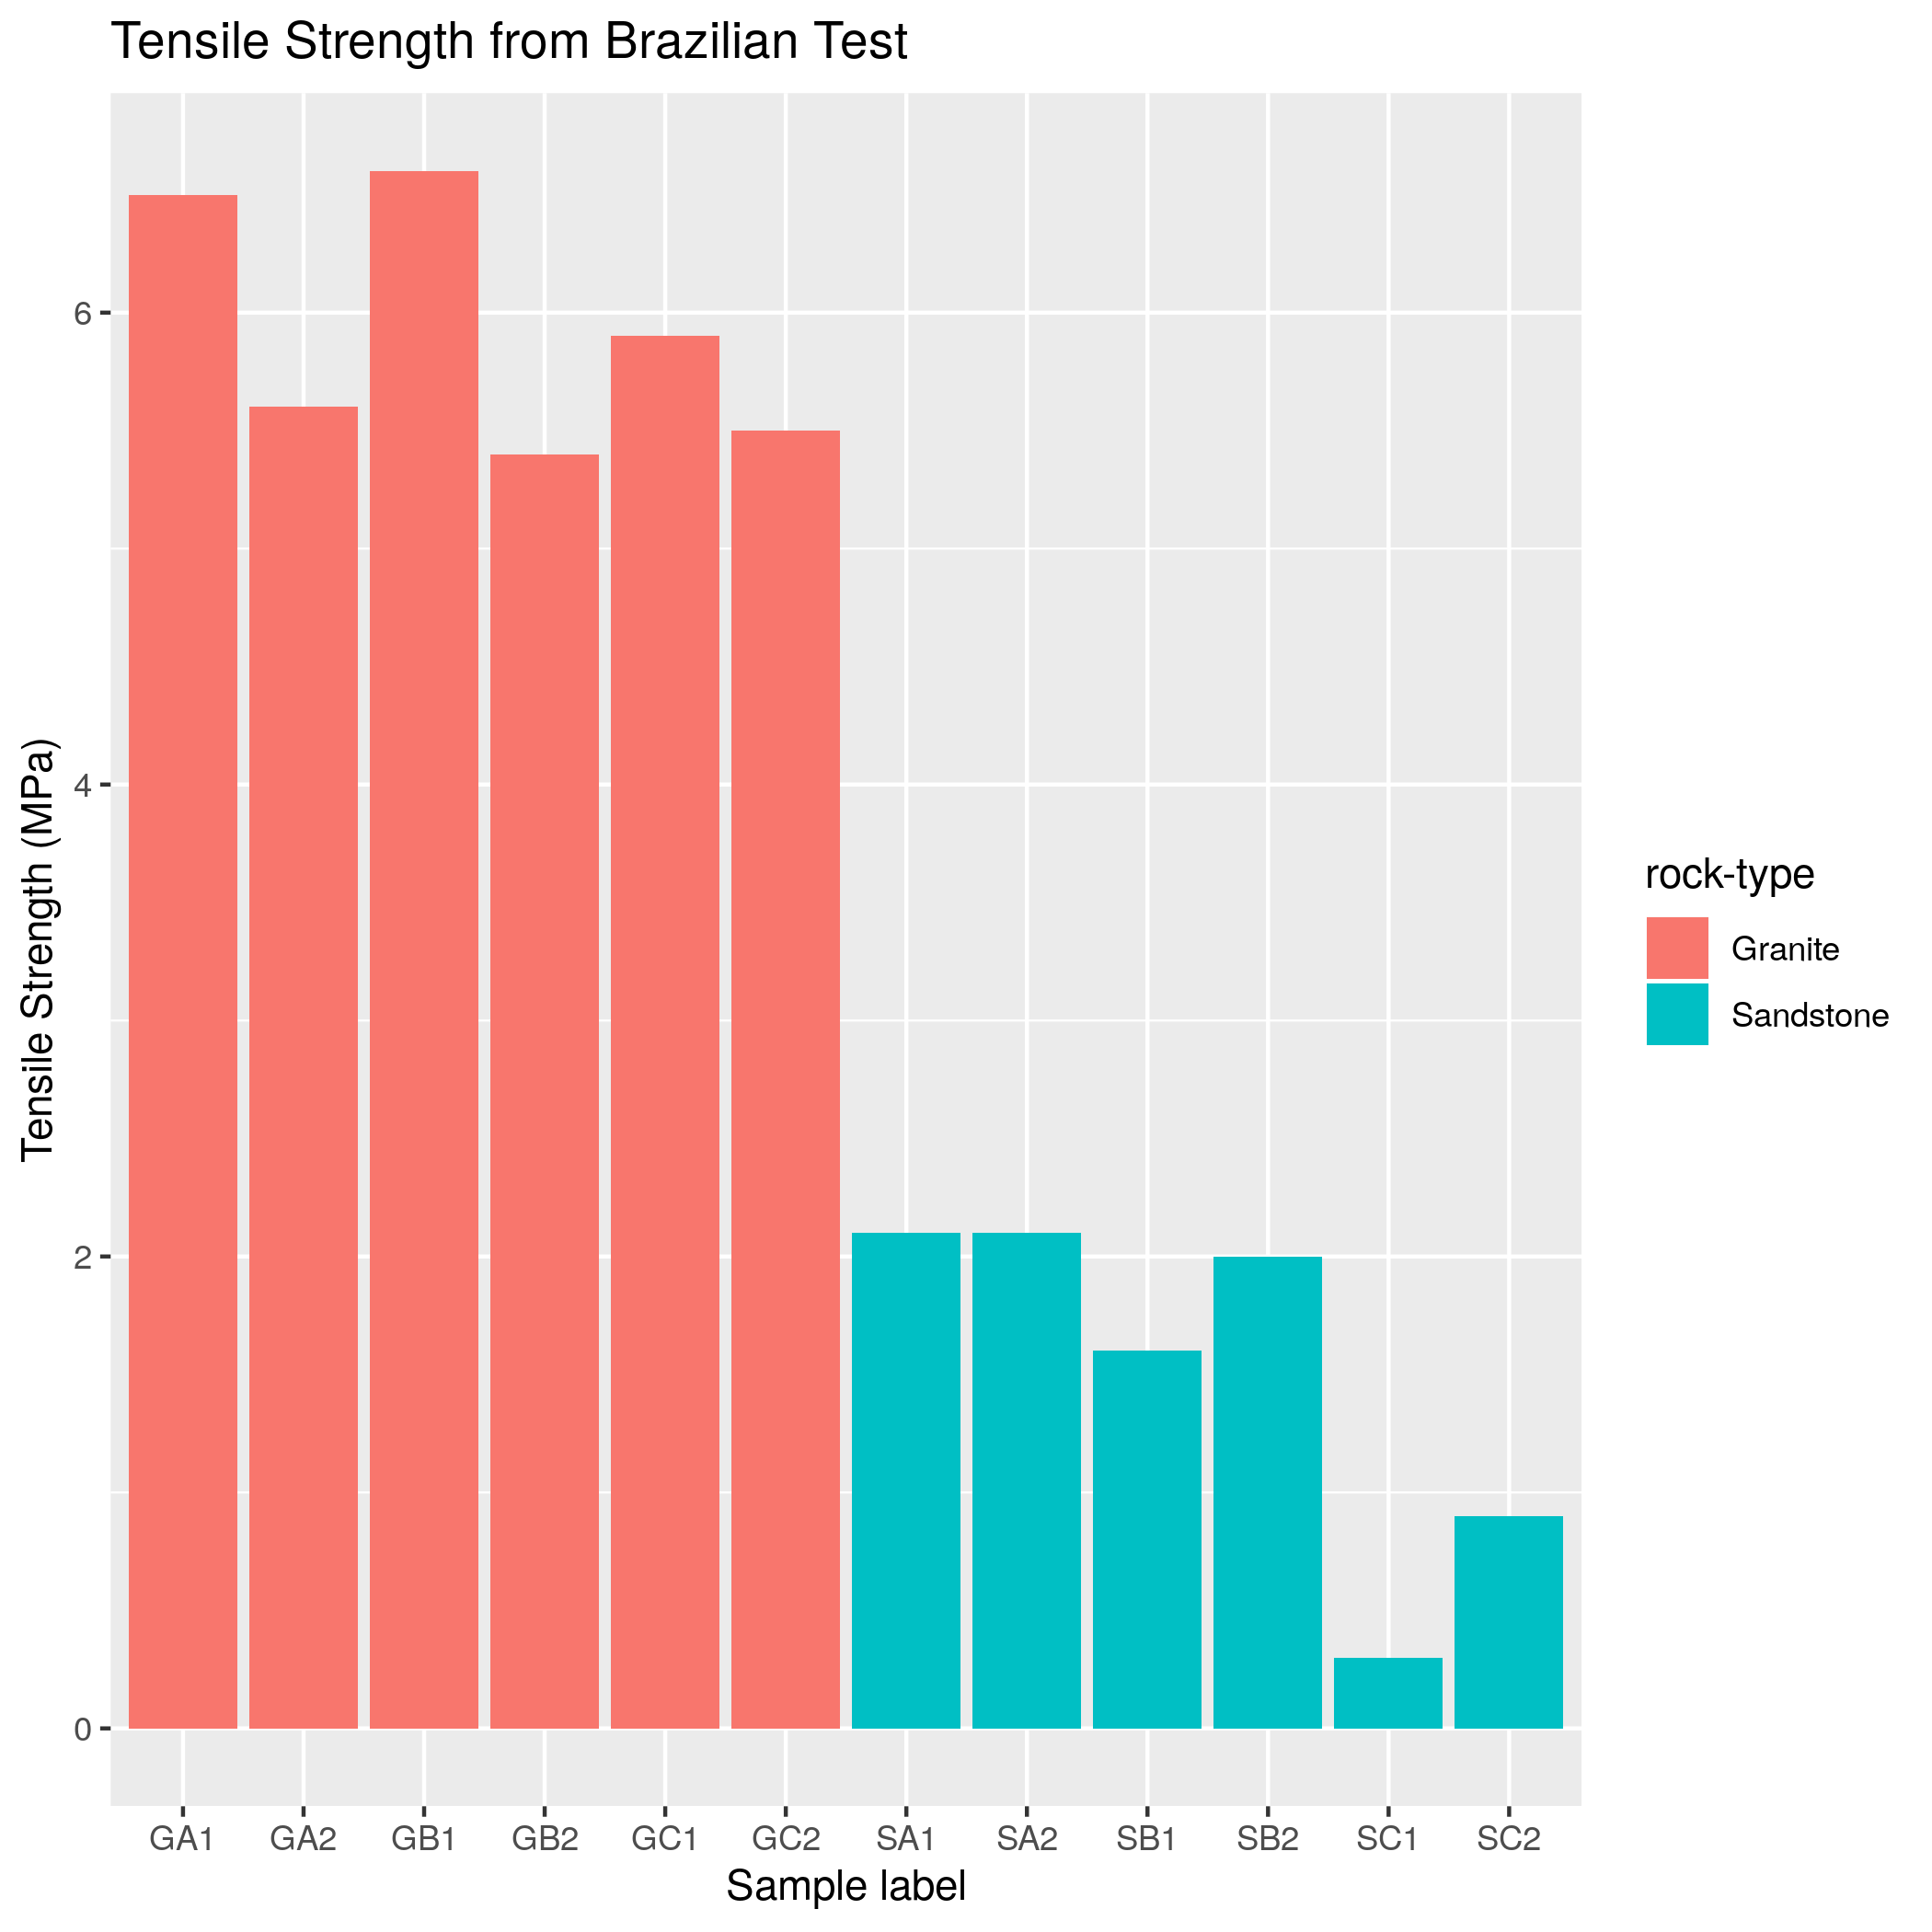
\includegraphics[width=0.7\linewidth]{brazilian.png}
    \caption{Brazilian test tensile strength results}
    \label{fig:brazilian-results}
\end{figure}

\pagebreak

\bibliographystyle{ans}
\printbibliography

\end{document}
